\documentclass{ucalgthes1}   
\usepackage[letterpaper,top=1in, bottom=1.22in, left=1.40in, right=0.850in]{geometry}
\usepackage{fancyhdr}
\fancyhead{}
\fancyfoot{}
\renewcommand{\headrulewidth}{0pt}
\fancyhead[RO,LE]{\thepage}  
\usepackage{hyperref}

\usepackage{algorithm}
\usepackage{algorithmic}
\usepackage{amsfonts}
\usepackage{amsmath}
\usepackage{amssymb}
\usepackage{amsthm}
\usepackage{comment}
\usepackage{float}
\usepackage{graphics}

\theoremstyle{plain}
\newtheorem{thm}{Theorem}[section]
\newtheorem{lemma}[thm]{Lemma}
\newtheorem{prop}[thm]{Proposition}
\newtheorem{cor}[thm]{Corollary}
\theoremstyle{definition}
\newtheorem{defn}[thm]{Definition}

\usepackage{eqparbox}
\renewcommand{\algorithmiccomment}[1]{\hfill\eqparbox{COMMENT}{#1}}
\renewcommand{\algorithmicrequire}{\textbf{Input:}}
\renewcommand{\algorithmicensure}{\textbf{Output:}}

\DeclareMathOperator*{\argmax}{arg\,max}
\DeclareMathOperator*{\argmin}{arg\,min}
\newcommand{\CC}{\mathbb{C}}
\newcommand{\NN}{\mathbb{N}}
\newcommand{\RR}{\mathbb{R}}
\newcommand{\KK}{\mathbb{K}}
\newcommand{\MM}{\mathcal{M}}
\newcommand{\OO}{\mathcal{O}}
\newcommand{\ZZ}{\mathbb{Z}}
\newcommand{\QQ}{\mathbb{Q}}
\newcommand{\NP}{\textrm{NP}}
\newcommand{\RRgtz}{\mathbb{R}_{>0}}
\newcommand{\ZZgtz}{\mathbb{Z}_{>0}}
\newcommand{\ZZgez}{\mathbb{Z}_{\ge 0}}
\newcommand{\QQgtz}{\mathbb{Q}_{>0}}
\newcommand{\QQgez}{\mathbb{Q}_{\ge 0}}
\newcommand{\matrixto}[2]{\left[ \begin{array}{rr} #1 & #2 \end{array} \right]}
\newcommand{\matrixot}[2]{\left[ \begin{array}{r} #1 \\ #2 \end{array} \right]}
\newcommand{\matrixtt}[4]{\left[ \begin{array}{rr} #1 & #2 \\ #3 & #4 \end{array} \right]}
\newcommand{\ntoinfty}{\lim_{n \rightarrow \infty}}
\newcommand{\floor}[1]{\left\lfloor #1 \right\rfloor}
\newcommand{\ceil}[1]{\left\lceil #1 \right\rceil}
\newcommand{\amax}{a_\textrm{max}}
\newcommand{\bmax}{b_\textrm{max}}

\begin{document}

\setcounter{chapter}{2}
\chapter{Exponentiation}
\label{chap:exponentiation}

Given a group $G$, an element $g \in G$, and an integer $n$, computing $g^n$ is a common operation and is known as exponentiation.  Diffie-Hellman key exchange is an example that uses exponentiation whereby two parties can jointly establish a shared secret key over an insecure channel.  An application discussed in detail in this thesis is that of computing the order of a group element.  Our approach is to exponentiate a group element to the product, $P$, of several small primes.  The result is an element whose order is likely to not be divisible by any of these primes. The order of this new element is then computed using a variant of Shanks' baby-step giant-step algorithm where only powers relatively prime to $P$ are computed.  Determining the order of an element can be useful in computing the structure of a group, or in factoring an integer associated with a group.  Being able to exponentiate faster implies that the larger operation can complete more quickly.

In Sections \ref{section:binary} and \ref{section:naf} we discuss standard exponentiation techniques that rely on a base 2 representation of the exponent.  In Section \ref{section:dbns} we introduce double-base number systems, which, as the name implies, are number systems that make use of multiple bases in the representation of a number.  We pay particular attention to double-base representations that use bases 2 and 3, since in our implementation of ideal class group arithmetic the cost of squaring is less than the cost of multiplying, and the cost of cubing is less than the cost of multiplying an element with its square. For this reason, we distinguish between the number of multiplications, squares, and cubes in an algorithm. In Section \ref{section:dbnsMethods} we discuss some methods to compute double-base representations found in the literature.  


%%%%%%%%%%%%%%%%%%%%%%%%%
% BINARY EXPONENTIATION %
%%%%%%%%%%%%%%%%%%%%%%%%%
\bigbreak
\section{Binary Exponentiation}\label{section:binary}
Perhaps the simplest method of exponentiation is that of binary exponentation.  Let $g$ be an element in the group $G$ and $n$ be a positive integer.  We want to compute $g^n \in G$.  We first represent $n$ in binary as
\[
	n = \sum_{i=0}^{\floor{log_2 n}} b_i 2^i
\]
where $b_i \in \{0, 1\}$ such that $b_i$ represents the $i^{\textrm{th}}$ bit of $n$.   We compute $g^{2^i}$ by repeated squaring of $g$ and compute $g^n$ by computing
\[
	g^n = \prod_{i=0}^{\floor{log_2 n}} g^{b_i 2^i}.
\]
This description is known as right-to-left binary exponentiation because the result is computed by generating the terms of the product from low order to high order.  The left-to-right variant evaluates the bits of the exponent $n$ from high order to lower order by repeatedly squaring an accumulator and multiplying this with the base element $g$ when $b_i = 1$.  The left-to-right variant has the advantage that one of the values in the multiplication, namely $g$, remains constant throughout the evaluation.  There also exist windowed variants where $g^w$ is precomputed for each $w$ in some window $0 \le w \le 2^k$ for some $k$ (typically chosen to be cache efficient). The exponent $n$ is then expressed in base $2^k$.  There are numerous sources discussing windowed variants such as (TODO) but we do not discuss these variants further here.

Binary exponentiation algorithms require $\floor{log_2 n}$ squarings and on average $\floor{log_2 n}/2$ multiplications, since a multiplication is only necessary when $b_i = 1$ and the probability of $b_i = 1$ is 1/2.

%%%%%%%%%%%%%%%%%%%%%%
% NAF EXPONENTIATION %
%%%%%%%%%%%%%%%%%%%%%%
\bigbreak
\section{Non-Adjacent Form Exponentiation}\label{section:naf}

The Non-Adjacent Form (NAF) of an integer is a \emph{signed} base two representation such that no two non-zero terms in the representation are adjacent. Each integer, $n$, has a unique representation in non-adjacent form. Formally, an integer $n$ is represented such that
\[
	n = \sum_{i=0}^{\floor{log_2 n}+1} s_i 2^i
\]
where $s_i \in \{0, 1, -1\}$ and $s_i \cdot s_{i+1} = 0$. For example, suppose $n = 23814216$.  In binary we have
\begin{equation}\label{eq:binaryEg}
	23814216 = 2^3+2^6+2^{13}+2^{14}+2^{16}+2^{17}+2^{19}+2^{21}+2^{22}+2^{24}
\end{equation}
and in non-adjacent form we have
\begin{equation}\label{eq:nafEg}
	23814216 = 2^3+2^6-2^{13}-2^{15}-2^{18}-2^{20}-2^{23}+2^{25}.
\end{equation}
Similar to the binary case, we can compute $g^n$ using
\[
	g^n = \prod _{i=0}^{\floor{log_2 n}+1} g^{s_i 2^i}.
\]
Since $s_i$ can be $-1$ and inversion can be expensive, we can instead compute the product as
\[
	g^n = \left( \prod_{i : s_i=1} g^{2^i} \right) \cdot \left( \prod_{i : s_i=-1} g^{2^i} \right)^{-1}
\]
which requires at most one inversion.

A typical method to compute the non-adjacent form of an integer $n$ is to inspect $n$ two bits at a time from least significant to most significant.  Let $n=\sum b_i2^i$ be the binary representation of $n$ and let $j=0$.  If the bit pattern $\langle b_{j+1}, b_j \rangle = 01$, then let $s_j = 1$ and subtract $2^j$ from $n$.  If $\langle b_{j+1}, b_j \rangle = 11$, then let $s_j = -1$ and add $2^j$ to $n$.  When the bit pattern $\langle b_{j+1}, b_j \rangle$ is $00$ or $10$, let $s_j = 0$. Next, increment $j$ and repeat while $n \ne 0$.

In our experiments, we use a variation of the above, originally due to Reitwiesner \cite{reitwiesner1960}, that maintains a carry flag $c$.  Instead of adding $2^i$ to $n$, we set $c = 1$, and instead of subtracting $2^i$ from $n$, we set $c = 0$.  When inspecting $n$ two bits at a time, we consider the bit pattern $(m+c) \bmod 4$ where $m = 2 b_{i+1} + b_i$.  For large enough $n$, the cost of addition and subtraction is reduced from $O(\log n)$ to $O(1)$.  See Algorithm \ref{alg:nafR2LImmutable}.

% R2L NAF EXPONENTIATION
\begin{algorithm}[h]
\caption{Computes $g^n$ using right-to-left non-adjacent form. Reitwiesner \cite{reitwiesner1960}}
\label{alg:nafR2LImmutable}
\begin{algorithmic}[1]
\REQUIRE $g \in G, n \in \ZZgez$
\STATE $c \gets 0$ \COMMENT{carry flag}
\STATE $T \gets g$ \COMMENT{invariant: $T = g^{2^i}$}
\STATE $R \gets 1_G$
\STATE $i \gets 0$
\WHILE {$n \ge 2^i$}
	\IF {$\floor{n/2^i}+c \equiv 1 \pmod 4$}
		\STATE $R \gets R \cdot T$
		\STATE $c \gets 0$
	\ELSIF {$\floor{n/2^i}+c \equiv 3 \pmod 4$}
		\STATE $R \gets R \cdot T^{-1}$
		\STATE $c \gets 1$
	\ENDIF
	\STATE $T \gets T^2$
	\STATE $i \gets i+1$
\ENDWHILE
\IF {$c=1$} \STATE $R \gets R \cdot T$ \ENDIF
\RETURN $R$
\end{algorithmic}
\end{algorithm}

A particular advantage of a non-adjacent form exponentiation over a binary exponentiation is the number of operations required.  While the binary method requires $\floor{\log_2 n}$ squares and on average $\floor{\log_2 n}/2$ multiplications, a non-adjacent form exponentiation requires at most $\floor{\log_2 n}+1$ squares and on average $(\floor{\log_2 n}+1)/3$ multiplications.  To see this, recall that non-adjacent form requires that no two non-zero terms be adjacent.  Consider any two adjacent terms.  The possible outcomes are $(0,0)$, $(s, 0)$, or $(0, s$) where $s \in \{-1, 1\}$. This means that 2/3 of the time, 1/2 of the terms will be non-zero, and so the probability of any given term being non-zero is 1/3.


%%%%%%%%
% DBNS %
%%%%%%%%
\bigbreak
\section{Double-Base Number Systems}\label{section:dbns}

A significant advantage of non-adjacent form over a binary representation is that on average the number of non-zero terms (the density of the representation) is lower.  We can achieve an even lower density on average when we extend the representation to a signed double-base number system (DBNS).  Binary and non-adjacent form are both base 2 number systems.  In the case of a double base number system, as the name suggests, we use two bases.  This system was first introduced by Dimitrov and Cooklev \cite{Dimitrov1995}.  Given two coprime integers $p$ and $q$ and some integer $n$, we represent $n$ as the sum and difference of the product of powers of $p$ and $q$,
\begin{equation}\label{eq:generalDbnsForm}
	n = \sum_{i=1}^k s_i p^{a_i} q^{b_i}
\end{equation}
where $s_i \in \{-1, 1\}$ and $a_i, b_i, k \in \ZZgez$.

Since this thesis focuses on exponentiation in the ideal class group, and since we can compute the square of an element faster than multiplying it with itself, and we can compute the cube of an element faster than multiplying its square with itself, we will be particularly interested in bases $p=2$ and $q=3$.  In other words, we will focus on representations of $n$ such that $n = \sum s_i 2^{a_i} 3^{b_i}$.

As an example of a 2,3 double-base representation, consider the number $n=23814216$ again.  Given the bases $p=2$ and $q=3$, \emph{one} possible representation of $n$ is
\begin{equation}\label{eq:chainedEg1}
	23814216 = 2^3 3^3 - 2^4 3^5 + 2^5 3^6  + 2^7 3^7  + 2^9 3^8 + 2^{10} 3^9.
\end{equation}
Another possible representation is
\begin{equation}\label{eq:chainedEg2}
	23814216 = 2^3 3^2 -2^{13} 3^2 +2^{15} 3^6.
\end{equation}
Double-base number systems are highly redudant, and different representations will trade off between cubings, squarings, and the number of terms.  The best representation, in some sense, will depend on the needs of the application.  Later, we shall see some algorithms that take this into account, but many are designed to either find representations quickly, of a special form, or with few terms.

Recall, the binary representation \eqref{eq:binaryEg}, non-adjacent form \eqref{eq:nafEg}, and a 2,3 double-base representation \eqref{eq:chainedEg2} of 23814216 were
\begin{align*}
	23814216 &= 2^3+2^6+2^{13}+2^{14}+2^{16}+2^{17}+2^{19}+2^{21}+2^{22}+2^{24}, & \mbox{using binary} \\
	23814216 &= 2^3+2^6-2^{13}-2^{15}-2^{18}-2^{20}-2^{23}+2^{25}, & \mbox{using NAF} \\
	23814216 &= 2^3 3^2 -2^{13} 3^2 +2^{15} 3^6. & \mbox{using 2,3 DBNS}
\end{align*}
The binary representation has 10 terms, while the non-adjacent form has only 8 terms.  The 2,3 representation given above contains only three terms.  While a non-adjacent form has in expectation $\floor{\log_2 n}/3$ terms and a binary representation has in expectation $\floor{\log_2 n}/2$ terms, both are bounded by $O(\log n)$ in the number of terms.  Both Dimitrov et al \cite{Dimitrov2008} and Ciet and Sica \cite{Ciet2005} give algorithms for 2,3 double-base representations, where they prove that the number of terms is bounded by $O(\log n / \log \log n)$.  For this reason, many algorithms focus on reducing the number of terms in a 2,3 representation.   Naturally, the time to compute a 2,3 double-base exponentiation is further reduced if the corresponding cost to compute $g^2$ is less than the cost to compute $g \cdot g$, or the cost to compute $g^3$ is less than the cost to compute $g^2 \cdot g$. 

%%%%%%%%%%%%%%%%%%%
\bigbreak
\subsection{Chains}

One way to classify algorithms that compute 2,3 representations is by the constraints placed on the \emph{partition} of an integer $n$.  For an example of a partition, consider the 2,3 representation of $23814216 = 2^3 3^2 -2^{13} 3^2 +2^{15} 3^6$.  The terms $2^3 3^2$, $2^{13} 3^2$, and $2^{15} 3^6$ when monotonically increasing by absolute value is a partition of the integer $23814216$.  

\begin{defn}
A partition of an integer $n = x_1 \pm x_2 \pm \cdots \pm x_k$ is \emph{chained} if every term $x_i$ divides every term $x_j$ for $i < j$ and $x_i \le x_j$. A partition is said to be \emph{strictly chained} if it is chained and $x_i$ is \emph{stricly} less than $x_j$ for each $i < j$.
\end{defn}

\noindent
Binary and non-adjacent form are special types of strictly chained partitions, since for any two non-zero terms where $i < j$, we have $x_i = 2^i$, $x_j = 2^j$, $ x_i ~|~ x_j$, and $x_i < x_j$.  The 2,3 representation of $23814216 = 2^3 3^2 - 2^{13} 3^2 + 2^{15} 3^6$ is another example of a strictly chained partition, since $2^3 3^2 ~|~ 2^{13} 3^2 ~|~ 2^{15} 3^6$.

% EXPONENTIATE USING A CHAIN
\begin{algorithm}[h]
\caption{Computes $g^n$ given $n$ as a chained 2,3 partition. TODO: Cite something.}
\label{alg:expWithChain}
\begin{algorithmic}[1]
\REQUIRE $g \in G,$ 
$n = \sum_{i=1}^k s_i2^{a_i}3^{b_i},$ \\
$s_1,...,s_k \in \{-1, 1\},$ 
$0 \le a_1 \le ...\le a_k \in \ZZ,$ 
$0 \le b_1 \le ... \le b_k \in \ZZ.$
\STATE $i \gets 1$
\STATE $a \gets 0$ \COMMENT{current power of 2}
\STATE $b \gets 0$ \COMMENT{current power of 3}
\STATE $T \gets g$ \COMMENT{loop invariant: $T = g^{2^a 3^b}$}
\STATE $R \gets 1_G$
\WHILE {$i \le k$}
	\WHILE {$a < a_i$}
		\STATE $T \gets T^2, a \gets a + 1$
	\ENDWHILE
	\WHILE {$b < b_i$}
		\STATE $T \gets T^3, b \gets b + 1$
	\ENDWHILE
	\STATE $R \gets R \cdot T^{s_i}$ \COMMENT{compose with $T$ or $T^{-1}$}
	\STATE $i \gets i + 1$
\ENDWHILE
\RETURN $R$
\end{algorithmic}
\end{algorithm}

The benefit of restricting 2,3 representations to chained representations is the ease with which one can compute $g^n$ when $n$ is given as a chain.  For example $g^{23814216} = g^{2^3 3^2 - 2^{13} 3^2 + 2^{15} 3^6}$ can be computed by first computing $x_1 = g^{2^3 3^2}$, $x_2 = {x_1}^{2^{10}}$, $x_3 = {x_2}^{2^2 3^4}$, and finally $g^{23814216} = \left(x_1 \cdot x_3\right) \cdot \left(x_2\right)^{-1}$.  Algorithm \ref{alg:expWithChain} can be used to compute $g^n$ for $g \in G$ and $n$ given as a chained 2,3 representation.  The cost of algorithm \ref{alg:expWithChain} is as follows: Let $n$ be defined as $\sum s_i 2^{a_i} 3^{b_i}$, let $max_a = \max \{a_1,...,a_k\}$, and let $max_b = \max \{b_1,...,b_k\}$.  Then we require $max_a$ squares, $max_b$ cubes, $k-1$ multiplications, and at most one inverse.  Since $x_i ~|~ x_{i+1}$, we need only retain $x_i$ in order to compute $x_{i+1}$, and so exponentiation and chain generation can easily be interleaved. For this reason, many algorithms that find 2,3 representations constrain these representations to be chains.  Section \ref{section:dbnsMethods} discusses some algorithms for simultaneously generating and exponentiating with such chains.



%%%%%%%%%%%%%%%%%%%%%%%%%%%%%%%%%%%%%%%%%%%%%%%%%%%%%%%
\bigbreak
\subsection{Exponentiating general 2,3 representations}

Another class of algorithms compute representations without the constraint that larger terms be divisible by smaller terms.  Given a general 2,3 representation for an integer $n = \sum s_i 2^{a_i} 3^{b_i}$, M\'{e}loni and Hasan \cite[Section 3.2]{Meloni2009} use a modification of Yao's Algorithm to achieve the same bound on the number of operations as in algorithm \ref{alg:expWithChain}, but with a bound of $O(\min \{max_a, max_b\})$ on the memory used.  Suppose $max_b < max_a$.  We require the terms to be labelled and sorted such that $a_1 \ge ... \ge a_k$.  The algorithm works by precomputing a table of $T_b = g^{3^b}$ for $0 \le b \le max_b$.  Let $i=1$ and begin with the first term $s_i2^{a_i}3^{b_i}$.  We look up $T_{b_i} = g^{3^{b_i}}$ and, after applying the sign $s_i$, we multiply ${T_{b_i}}^{s_i}$ with the running result.  Let $a_\Delta = a_i - a_{i+1}$ when $i < k$ and $a_\Delta = a_k$ when $i = k$.  It then squares the running result $a_\Delta$ times.  The algorithm removes the term $s_i2^{a_i}3^{b_i}$ from the list of terms, and continues in this way with the next largest $a_i$.  The algorithm terminates when there are no more terms in the list.  Algorithm  \ref{alg:yaos} gives pseudo-code for this approach and requires $O(max_b)$ memory.  When $max_a < max_b$, we use a related algorithm that requires the terms to be sorted such that $b_1 \ge ... \ge b_k$; it precomputes $T_a = g^{2^a}$ for $0 \le a \le max_a$ and works similar to Algorithm \ref{alg:yaos} but with cubing and squaring appropriately swapped.

% EXPONENTIATE USING YAO'S
\begin{algorithm}[h]
\caption{Computes $g^n$ given $n$ in 2,3 representation. M\'{e}loni \cite[Section 3.2]{Meloni2009}.}
\label{alg:yaos}
\begin{algorithmic}[1]
\REQUIRE $g \in G,$ 
$n = \sum_{i=1}^k s_i2^{a_i}3^{b_i},$ \\
$s_1,...,s_k \in \{-1, 1\},$ 
$a_1 \ge ... \ge a_k \in \ZZgez,$ 
$b_1,...,b_k \in \ZZgez.$
\STATE $T_b \gets g^{3^b}$ for $0 \le b \le \max \{ b_1, ..., b_k \}$ \COMMENT{by repeated cubing}
\STATE $R \gets 1_G$
\STATE $i \gets 1$
\WHILE {$i < k$}
	\STATE $R \gets R \cdot {T_{b_i}}^{s_i}$ \COMMENT{compose with $T_{b_i}$ or ${T_{b_i}}^{-1}$}
	\STATE $a_\Delta \gets a_i - a_{i+1}$
	\STATE $R \gets R ^ {2^{a_\Delta}}$ \COMMENT{by squaring $a_\Delta$ number of times}
	\STATE $i \gets i + 1$
\ENDWHILE
\STATE $R \gets R \cdot {T_{b_k}}^{s_k}$
\STATE $R \gets R ^ {2^{a_k}}$ \COMMENT{by squaring $a_k$ number of times}
\RETURN $R$
\end{algorithmic}
\end{algorithm}

For example, the 2,3 representation $23814216 = 2^{15} 3^6 - 2^8 3^5 - 2^4 3^6 + 2^3 3^3$ is sorted by decreasing $a_i$.  The algorithm first computes $T_b = g^{3^b}$ for $0 \le b \le 6$.  Note that it is sufficient to store only the values of $g^{3^{b_i}}$ that actually occur in terms (in this example, we need only store $T_3$, $T_5$, and $T_6$).  Let $R_j$ represent the partial exponentiation of the first $j$ terms with the largest $a_i$ such that $g^{2^{a_{j+1}}}$ is factored out.  Let $R_0 = 1_G$.  In this example, we compute 
\begin{align*}
	R_1 &= \left( T_6 \right)^{2^7} &&\Rightarrow g^{2^7 3^6}, \\
	R_2 &= \left( R_1 {T_5}^{-1} \right)^{2^4} &&\Rightarrow g^{-2^4 3^5 + 2^{11} 3^6}, \\
	R_3 &= \left( R_2 {T_6}^{-1} \right)^{2^1} &&\Rightarrow g^{-2^1 3^6 -2^5 3^5 + 2^{12} 3^6}, \\
	R_4 &= \left( R_3 T_3 \right) ^ {2^3} &&\Rightarrow g^{2^3 3^3 -2^4 3^6 -2^8 3^5 + 2^{15} 3^6},
\end{align*}
as depicted by figure \ref{fig:yao1}.  The result of the computation is $R_4 = g^{23814216}$.  

% figure of exponentiating 23814216 with unchained representation
\begin{figure}[H]
\centering
\includegraphics{yao1}
\caption{The construction of $2^{15} 3^6 - 2^8 3^5 - 2^4 3^6 + 2^3 3^3$ using algorithm \ref{alg:yaos}.  Steps are executed from left-to-right, top-to-bottom.}
\label{fig:yao1}
\end{figure}


%%%%%%%%%%%%%%%%%%%%%%%%%%%%%%%%%%%%%%%%%%%%%%%%%%%%
% METHODS FOR COMPUTING 2,3 CHAINS/REPRESENTATIONS %
%%%%%%%%%%%%%%%%%%%%%%%%%%%%%%%%%%%%%%%%%%%%%%%%%%%%
\bigbreak
\section{Methods for computing 2,3 Chains/Representations}
\label{section:dbnsMethods}

Factors influencing the speed of a 2,3 exponentiation are the time to generate the 2,3 chain or representation, and the cost of group operations such as compose, square, and cube. If the exponent is a constant, then we can precompute the chain or representation. Here we discuss some methods from the literature: the first generates strict chains from low order to high order (right-to-left), the second generates representations (chained or unchained) from high order to low order (left-to-right), and the last generates strict chains using a tree-based approach.  For an integer $n$, each successive method introduced below typically requires more time to generate a 2,3 representation, but the representation typically has fewer terms.  As such, these methods show a trade off between the time spent computing a representation and the time spent exponentiating with the representation.  None of these methods take the relative cost of composing, squaring, or cubing into account.  In Chapter \ref{chap:idealExponentiationExperiments} we will look at variations of these algorithms that generate reprensentations that attempt to minimize the cost of exponentation given the relative costs of group operations.

%%%%%%%%%%%%%%%%%%%%%%%%%%%%%%%%%%%%%%%%%%%%%%%%%%%%%%%%%%%%%%%%
\bigbreak
\subsection{Right-to-Left Chains (from low-order to high-order)}
\label{subsec:rtolchains}

The first method we present computes a strictly chained 2,3 partition that is generated from low order to high order and is based on Ciet et al \cite{Ciet2006}.  Consider the technique for binary exponentiation that computes from low order to high order.  We can give a recursive algorithm by defining a function such that given an element $g \in G$ and an integer $n$:
\begin{align*}
\textrm{bin}(g, n) &= \begin{cases}
               1 & \textrm{if $n = 0$} \\
               {\textrm{bin}(g, n/2)}^2 & \textrm{if $n \equiv 0 \pmod 2$} \\
               \textrm{bin}(g, n-1) \cdot g & \textrm{if $n \equiv 1 \pmod 2$}. \\
	       \end{cases}
\end{align*}

\noindent
This algorithm will repeatedly remove factors of 2 from $n$.  When $n$ is not divisible by 2, it subtracts 1 such that the input to the recursive call will be divisible by 2.  The recursion terminates with the base case of $n=0$.

We can extend this concept to a 2,3 number system.  We will repeatedly remove factors of 2 from $n$, then repeatedly remove factors of 3 from $n$.  At this point, either $n \equiv 1 \pmod 6$ or $n \equiv 5 \pmod 6$.  When $n \equiv 1 \pmod 6$, we recurse on $n-1$ and the input will be divisible by both 2 and 3.  When $n \equiv 5 \pmod 6$, we recurse on $n+1$.  Again, the input to the recursive call will be divisible by both 2 and by 3.  The function below performs a 2,3 exponentiation recursively:
\newcommand{\rtol}{\textrm{r}_2\textrm{l}}
\begin{align*}
\rtol(g, n) &= \begin{cases}
               1 & \textrm{if $n = 0$} \\
               {\rtol(g, n/2)}^2 & \textrm{if $n \equiv 0 \pmod 2$} \\
               {\rtol(g, n/3)}^3 & \textrm{if $n \equiv 0 \pmod 3$} \\
               \rtol(g, n-1) \cdot g & \textrm{if $n \equiv 1 \pmod 3$} \\
               \rtol(g, n+1) \cdot g^{-1} & \textrm{if $n \equiv 2 \pmod 3$} \\
	       \end{cases}
\end{align*}

Using this technique, we can devise a function to compute a strictly chained 2,3 partition of $n$ that corresponds to the group operations generated by $\rtol$. This is useful when recursion isn't possible, or when the exponent $n$ is a constant (since we can use precomputation to save time). Algorithm \ref{alg:rtolDbnsChain} computes the corresponding strictly chained 2,3 partition.  The idea is as follows: let $a = 0$, $b=0$, and $i=1$.  While $n > 0$, repeatedly remove factors of 2 from $n$ and increment $a$ for each factor of 2 removed. Then repeatedly remove factors of 3 from $n$ and increment $b$ for each factor of 3 removed. At this point, either $n \equiv 1 \pmod 6$ or $n \equiv 5 \pmod 6$ and so continue on $n-1$ or $n+1$ respectively.  When we continue on $n-1$, this corresponds to adding the current term, so we set $s_i=1$, and when we continue on $n+1$, this corresponds to subtracting the current term, so we set $s_i=-1$. Let $a_i = a$ and $b_i = b$ and then increment $i$ and then repeat this process while $n > 0$.  We can then use Algorithm \ref{alg:expWithChain} to compute the exponentiation given a strictly chained 2,3 partition. Additionally, since the terms $s_i2^{a_i}3^{b_i}$ are computed in increasing order for $i=1..k$, it is relatively straightforword to interleave the computation of the partition with the computation of the exponentiation for additional speed and memory savings.

% R2L 2,3 CHAIN
\begin{algorithm}[h]
\caption{Computes a 2,3 strictly chained representation from low order to high order. Ciet \cite{Ciet2006}.}
\label{alg:rtolDbnsChain}
\begin{algorithmic}[1]
\REQUIRE $n \in \ZZgez$
%\ENSURE $n=\sum_{i=1}^k s_i2^{a_i}3^{b_i}$ as a strictly chained partition.
\STATE $(a, b) \gets (0, 0)$
\STATE $i \gets 1$
\WHILE {$n > 0$}
	\WHILE {$n \equiv 0 \pmod 2$} 
		\STATE $n \gets n / 2, a \gets a + 1$
	\ENDWHILE
	\WHILE {$n \equiv 0 \pmod 3$}
		\STATE $n \gets n / 3, b \gets b + 1$
	\ENDWHILE
	\IF {$n \equiv 1 \pmod 3$}
		\STATE $n \gets n - 1, s \gets 1$
	\ELSIF {$n \equiv 2 \pmod 3$}
		\STATE $n \gets n + 1, s \gets -1$
	\ENDIF
	\STATE $(s_i, a_i, b_i) \gets (s, a, b)$
	\STATE $i \gets i + 1$
\ENDWHILE
\STATE $k \gets i$
\RETURN $(a_1, b_1, s_1), ..., (a_k, b_k, s_k)$
\end{algorithmic}
\end{algorithm}

To see the correctness of the above procedure, consider a modification to the recursive function $\rtol$ such that it returns a partition of the input $n$ as a list of terms $s_i2^{a_i}3^{b_i}$. When the result of the recursive call is squared, this corresponds to incrementing $a_i$ in each term of the list.  Similarly, when the result is cubed, this corresponds to incrementing $b_i$ in each term of the list. When the result is composed with $g$, we prepend a term of $+1$ to the partition, and when the result is composed with $g^{-1}$, we prepend a term of $-1$ to the partition. Note that since either $n \equiv 0 \pmod 2$ or $n \equiv 0 \pmod 3$ on each iteration of the loop, either $a$ will increase or $b$ will increase. Since every term $|s_i2^{a_i}3^{b_i}|$ is strictly less than $|s_j2^{a_j}3^{b_j}|$ when $i < j$, the partition is strictly chained.

%%%%%%%%%%%%%%%%%%%%%%%%%%%%%%%%%%%%%%%%%%%%%%%%%%%%%%%%%%%%%%%%
\bigbreak
\subsection{Left-to-Right Chains (from high-order to low-order)}

\newcommand{\greedyltor}{\textrm{greedy}}
\newcommand{\greedychain}{\textrm{greedy}'}
\newcommand{\greedybound}{\textrm{greedy}''}
\newcommand{\closest}{\textrm{closest}}

The previous section gave a procedure for generating a strictly chained 2,3 partition for an integer $n$ such that the terms were ordered from smallest absolute value to largest.  Here we present a greedy approach that generates the terms in order of the largest absolute value to the smallest. The general idea is to find a term, $s2^a3^b$, that is closest to the remaining target integer $n$ and then repeat on $n - s2^a3^b$.  Let $\closest(n) = s2^a3^b$ such that $(a,b) = \argmin_{(c,d)} \{ \left| |n| - 2^c3^d \right| : c,d \in \ZZgez \}$ where $s = -1$ when $n < 0$ and $s = 1$ otherwise. Note that $n$ may be negative. A recursive function to greedily compute a 2,3 representation is given as:
\begin{align*}
\greedyltor(n) &= \begin{cases}
              0 & \textrm{if $n = 0$} \\
              \closest(n) + \greedyltor(n - \closest(n)) & \textrm{otherwise}
          \end{cases}
\end{align*}

\noindent
Note that the representation generated may not be a chained partition, however, we can still use the representation to exponentiate a group element $g \in G$ using Algorithm \ref{alg:yaos}.

In order to generate a chained partition we restrict the maximum powers of 2 and 3 generated by the function $\closest$.  We bound $\closest$, such that it returns a triple as follows:
\[
\closest'(n, \amax, \bmax) = (s2^a3^b, a, b)
\]
where
\[
(a, b) =
\argmin_{(c,d)} \left\{\left| |n| - 2^c3^d \right| : c, d \in \ZZgez, c \le \amax, d \le \bmax \right\}
\]
and $s=-1$ when $n < 0$ and $s=1$ when $n > 0$. Our recursive function is then:
\begin{align*}
\greedychain(n, \amax, \bmax) &= \begin{cases}
        0 & \textrm{if $n = 0$} \\
        v + \greedychain(n - v, a, b) & \textrm{where $(v, a, b) = \closest'(n, \amax, \bmax)$}
    \end{cases}
\end{align*}

\noindent
We present pseudocode in Algorithm \ref{alg:greedyltor}. Note that on successive invocations of $\greedychain$, the absolute value of $v=|s2^a3^b|$ returned by $\closest'$ is monotonically decreasing.  Reversing the terms of the partition gives a chained 2,3 partition of $n$ that we can use to perform exponentiation using Algorithm \ref{alg:expWithChain}.

% GREEDY L2R
\begin{algorithm}[h]
\caption{Greedy left to right representations. Berth\'{e} and Imbert \cite{Berthe2009}.}
\label{alg:greedyltor}
\begin{algorithmic}[1]
\REQUIRE $n, \amax, \bmax \in \{\ZZgez, +\infty\}$ \COMMENT{$+\infty$ for unbounded $a$ or $b$}
\STATE $L \gets \textrm{empty list}$
\WHILE {$n \ne 0$}
	\STATE $(a, b) \gets \argmin_{(c, d)} \left\{\left||n| - 2^c3^d \right| : 0 \le c \le \amax, 0 \le d \le \bmax \right\}$
	\STATE $s \gets -1 \textrm{ when } n < 0 \textrm{ and } 1 \textrm{ otherwise}$
	\STATE $\textrm{push }(s, a, b) \textrm{ onto the front of } L$
	\STATE $\textrm{optionally set } (\amax, \bmax) \gets (a, b) \textrm{ when a chain is desired}$
	\STATE $n \gets n - s2^a3^b$
\ENDWHILE
\RETURN $L$
\end{algorithmic}
\end{algorithm}

To compute the 2,3 term closest to $n$, a straightforward approach is to compute the set 
\[
V = \{2^a3^b, 2^{a+1}3^b : 0 \le b \le \ceil{log_3|n|}, a=\floor{|n/(3^b)|} \},
\]
take the element $v \in V$ that is closest to $|n|$, and take $s \in \{-1, 1\}$ based on the sign of $n$, constraining $a$ and $b$ appropriately based on maximal values permitted. Since the set $V$ contains $O(\log |n|)$ elements, computing the term closest to $n$ by this method takes $\Omega(\log |n|)$ steps.  When $a$ and $b$ are not constrained, and we simply want to compute the 2,3 term closest to $n$, Berth\'{e} and Imbert \cite{Berthe2009} present a method that requires at most $O(\log \log |n|)$ steps. 

Naturally though, non-chained representations tend to have a lower density than chained representations but at the expense of requiring more memory to perform exponentiation.  Since we can exponentiate non-chained representations using Algorithm \ref{alg:yaos} and requiring memory proportional to the largest values of $a$ and $b$ in the representation, constraining $a$ and $b$ globally over the complete representation can result in representations that exponentiate more quickly in practice. In this case, recursive calls to $\greedychain$ use the original values of $\amax$ and $\bmax$ rather than further constraining $a$ and $b$ based on the values generated by $\closest'$.  Finding the best greedy representation is then a matter of iterating over $\amax$ and $\bmax$ and computing 2,3 representations costrained appropriately.  We will discuss approaches and results of this in Chapter \ref{chap:idealExponentiationExperiments}.



%%%%%%%%%%%%%%%%%%%%%%%%%
\bigbreak
\subsection{Pruned Trees}

The next technique for finding stricly chained 2,3 partitions was suggested by Doche and Habsieger \cite{Doche2008}. The idea is similar to the method for generating chains from right to left as described in Subsection \ref{subsec:rtolchains} above, but this technique differs by generating several possible values that may be further reduced by powers of 2 and 3. The procedure is given in Algorithm \ref{alg:dbnsTree}.  The idea is to maintain a tree, $T$, with at most $B$ leaf nodes. At each iteration, each leaf node $v \in T$ generates two new leaves, $v-1$ and $v+1$, which are then reduced as much as possible by removing factors of 2 and 3.  We then discard any duplicate nodes and all but the smallest $B$ elements generated. The path from the root to the first leaf with a value of 1 represents a chained 2,3 partition of the number $n$.

%%%%%%%%%%%%%
% DBNS TREE %
%%%%%%%%%%%%%
\begin{algorithm}[h]
\caption{Tree-Based Chained 2,3 Partitions. Doche and Habsieger \cite{Doche2008}.}
\label{alg:dbnsTree}
\begin{algorithmic}[1]
\REQUIRE $n \in \ZZgtz$
\STATE $T \gets$ a binary tree on the node $n$
\WHILE {no leaf is 1}
	\FORALL {leaf nodes $v \in T$}
		\STATE insert as a left child $(v - 1)$ with all factors of 2 and 3 removed
		\STATE insert as a right child $(v + 1)$ with all factors of 2 and 3 removed
	\ENDFOR
	\STATE discard any duplicate leaves
	\STATE discard all but the smallest $B$ leaves
\ENDWHILE
\RETURN the chained 2,3 partition generated by the path from the root to the first leaf node containing 1
\end{algorithmic}
\end{algorithm}

Empirically they found that $B=4$ was a good compromise between the length of the chain generated and the time to compute the chain. Larger values of $B$ sometimes produce chains with fewer terms, but take longer to compute. When the number for the target chain is known in advance and precomputation is permitted, a larger value of $B$ can be advantageous since this can lead to fewer terms, which can lead to a cheaper exponentiation.  The downside is that large values of $B$ can be prohibitively expensive even for precomputation when the integer $n$ is quite large.



\end{document}

